Para los casos de prueba o dataset, se hace uso del lenguaje de programación Python para facilitar la generación automática de datos en archivos \texttt{.txt}, los cuales se utilizan como datos de entrada para los programas \texttt{brute\_force.cpp} y \texttt{dynamic\_programming.cpp}.

El programa \textsc{generate\_datasets.py} genera automáticamente 5 archivos \texttt{.txt} para cada una de las tres categorías de casos de prueba definidas:

\subsubsection{Transpose Datasets}
En esta categoría se generan 5 archivos con el prefijo \texttt{input\_transpose}, enumerados del 1 al 5. Los strings en estos archivos se ordenan de menor a mayor longitud, y todos los problemas planteados pueden resolverse exclusivamente mediante operaciones de transposición. Sin embargo, no se garantiza que la solución óptima obtenida por los programas implique únicamente transposiciones, ya que esto dependerá de los costos asociados a cada operación y de si estas resultan más convenientes.

\subsubsection{Semi-Ordered Datasets}
En esta categoría, la mitad del string \( S1 \) será idéntica a la otra mitad del string \( S2 \). Esto permite observar cómo se comportan los enfoques algorítmicos de \textit{Fuerza Bruta} y \textit{Programación Dinámica} en casos parcialmente ordenados. Los archivos generados llevan el prefijo \texttt{input\_semiordered}.

\subsubsection{Disordered Datasets}
Por último, esta categoría contiene datasets donde \( S1 \) y \( S2 \) son completamente desordenados, generados de manera aleatoria. Los archivos generados llevan el prefijo \texttt{input\_disordered}. En este caso, es probable que el enfoque de \textit{Fuerza Bruta} tarde significativamente más tiempo en procesar strings con una longitud superior a 16 caracteres, debido al crecimiento exponencial de su árbol implícito de llamadas recursivas y la necesidad de explorarlo en profundidad.

Ver la siguiente \cref{fig:ejemplo-datasets}
\begin{figure}[H]
    \centering
    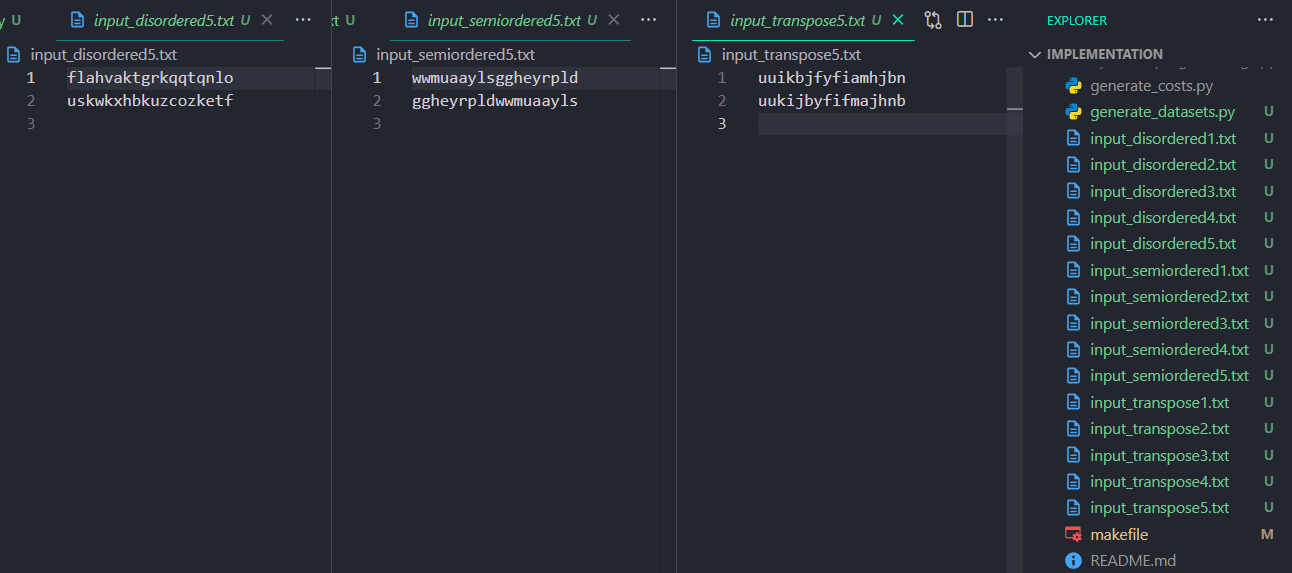
\includegraphics[width=1\linewidth]{Tarea_2&3//images/ejemplo_datasets.png}
    \caption{Ejemplo de los archivos .txt generados por el archivo \textit{generate\_datasets.py}.}
    \label{fig:ejemplo-datasets}
\end{figure}